\documentclass[handout]{beamer}

\usepackage{fontspec} 
% \usepackage{lsp-makros}
\useoutertheme{lsp}

\usepackage{lsptitle}
\usepackage{tikz}
\usetikzlibrary{positioning}
\def\two@digits#1{\ifnum#1<10 0\fi\number#1}
\def\mytoday{\two@digits{\number\day}.\two@digits{\number\month}.\number\year}


\usepackage{xspace,multicol}
\newcommand{\latex}{\LaTeX\xspace}


\newcounter{lastpagemainpart}
\footnotesep0pt
\renewcommand{\footnoterule}{}
\usefootnotetemplate{
  \noindent
  \insertfootnotemark\insertfootnotetext}

\let\beamerfn=\footnote
\renewcommand{\footnote}[1]{%
\let\oldfnsize=\footnotesize%
\let\footnotesize=\tiny%
\beamerfn<\thebeamerpauses->{#1}%
\let\footnotesize=\oldfnsize}


\date{2023-06-28}

\usepackage{eurosym}  
 
\renewcommand{\centerline}[1]{\hfill#1\hfill\hfill\mbox{}}


\title{Open Text Collections}
% \institute{}
\author[Nordhoff]{Sebastian Nordhoff\\Corpus Glosés: de la construction à l'exploitation automatique}



\begin{document}
\lspbeamertitle




\section{intro}
\frame{
\frametitle{Introduction}
%   \includegraphics[height=.2\textheight]{./path/to/graphicsfile}
  \includegraphics[height=\textheight]{jldc2008.png}
  \includegraphics[height=\textheight]{ldc.png}
  \begin{itemize}
    \item work on grammaticography since 2007
    \item Language Science Press since 2014
    \item starting 2023: open text collections
  \end{itemize}


}


\frame{
\frametitle{Boasian Trilogy:\\ publication options}
%   \includegraphics[height=.2\textheight]{./path/to/graphicsfile}
  \begin{itemize}
    \item
    \item
  \end{itemize}
      herleitung
          wörterbuch
          grammatik
}

\frame{
\frametitle{Existing platforms}
%   \includegraphics[height=.2\textheight]{./path/to/graphicsfile}
  \begin{itemize}
    \item  TILA
    \item pangloss
    \item doreco
    \item eopas
  \end{itemize}
}

\frame{
\frametitle{Open Text Collections}
%   \includegraphics[height=.2\textheight]{./path/to/graphicsfile}
  \begin{itemize}
    \item      open
    \item   prestigious
    \item   interoperable
    \item   start 15.9.
  \end{itemize}
}
\section{guiding principles}
\frame{
\frametitle{Guiding principles}
%   \includegraphics[height=.2\textheight]{./path/to/graphicsfile}
  \begin{itemize}
    \item  texts
    \item  edited
    \item  curated
    \item  data first
    \item  community
    \item  openness
    \item  prestige
  \end{itemize}
}
\section{input}

\frame{
\frametitle{Import}
%   \includegraphics[height=.2\textheight]{./path/to/graphicsfile}
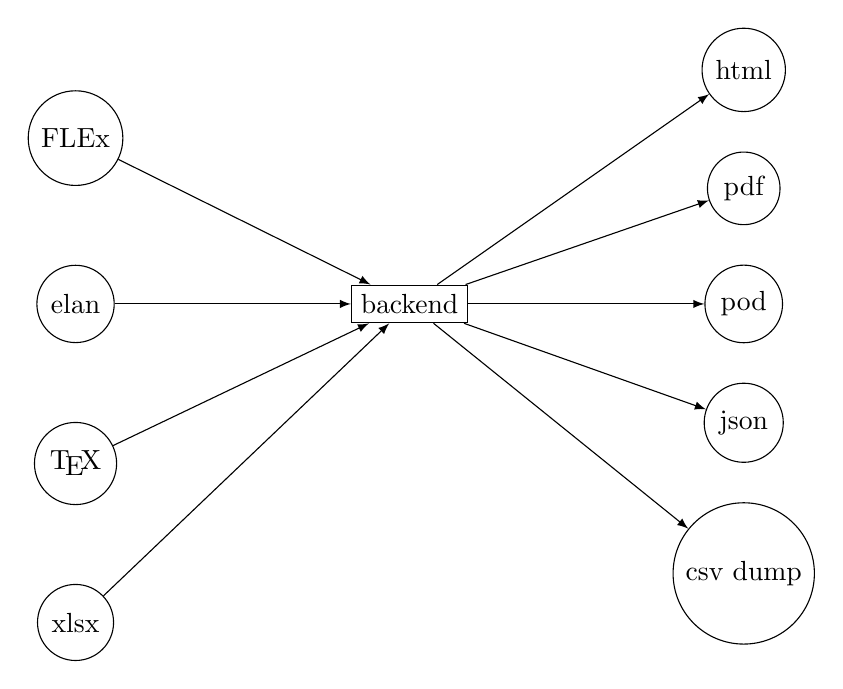
\begin{tikzpicture}
  \node(backend)[rectangle,draw]{backend};
  \node(elan)[circle,draw,left =3cm of backend]{elan};
  \node(flex)[circle,draw,above = 1cm of elan]{FLEx};
  \node(tex)[circle,draw,below = 1cm of elan]{\TeX};
  \node(xlsx)[circle,draw,below = 1cm of tex]{xlsx};
  \node(pod)[circle,draw,right = 3cm of backend]{pod};
  \node(pdf)[circle,draw,above = 5mm of pod]{pdf};
  \node(html)[circle,draw,above = 5mm of pdf]{html};
  \node(json)[circle,draw,below = 5mm of pod]{json};
  \node(csv)[circle,draw,below = 5mm of json]{csv dump};
\draw[-latex](elan)->(backend);
\draw[-latex](flex)->(backend);
\draw[-latex](tex) ->(backend);
\draw[-latex](xlsx)->(backend);
\draw[-latex](backend)->(pod);
\draw[-latex](backend)->(pdf);
\draw[-latex](backend)->(html);
\draw[-latex](backend)->(json);
\draw[-latex](backend)->(csv);
\end{tikzpicture}


  \begin{itemize}
    \item
    \item
  \end{itemize}
      import routine
          ELAN
              spracharchive
                  consistency
          FLEX
          tex


}


\frame{
\frametitle{Consistency}
%   \includegraphics[height=.2\textheight]{./path/to/graphicsfile}
  \begin{itemize}
    \item  20000 files under the sea
    \item
  \end{itemize}
}

\section{backend}

\frame{
\frametitle{Backend}
%   \includegraphics[height=.2\textheight]{./path/to/graphicsfile}
  \begin{itemize}
    \item
    \item
  \end{itemize}
      csv
}

\frame{
\frametitle{Frametitle3}
  \includegraphics[height=.2\textheight]{backend_csv.png}
}

\section{output}
\frame{
\frametitle{Output formats}
%   \includegraphics[height=.2\textheight]{./path/to/graphicsfile}
  \begin{itemize}
    \item
    \item
  \end{itemize}
      dump
          rdf
          json
      book
          pdf
              Amazon
          pod
      html
      querying
          imtvault
}

\section{workflow}

\frame{
\frametitle{GitHub}
%   \includegraphics[height=.2\textheight]{./path/to/graphicsfile}
  \begin{itemize}
    \item
    \item
  \end{itemize}
}

\frame{
\frametitle{Zenodo}
%   \includegraphics[height=.2\textheight]{./path/to/graphicsfile}
  \begin{itemize}
    \item
    \item
  \end{itemize}
}

\frame{
\frametitle{quality assurance}
%   \includegraphics[height=.2\textheight]{./path/to/graphicsfile}
  \begin{itemize}
    \item
    \item
  \end{itemize}
          technical review
          regional boards
}

\section{technical}
\frame{
\frametitle{Data model}
%   \includegraphics[height=.2\textheight]{./path/to/graphicsfile}
  \begin{itemize}
    \item
    \item
  \end{itemize}
      Data model
          three main tiers
              additional tiers
              CSVW
          csv
          json
          rdf
          Linked Data
}

\frame{
\frametitle{FAIR}
%   \includegraphics[height=.2\textheight]{./path/to/graphicsfile}
  \begin{itemize}
    \item
    \item
  \end{itemize}
          findable
              registered, linked, metadata
          accessible
              no paywalls
          interoperable
              many different formats
          reusable
              open license
}

\section{funding model}

\frame{
\frametitle{Fundin}
%   \includegraphics[height=.2\textheight]{./path/to/graphicsfile}
  \begin{itemize}
    \item
    \item
  \end{itemize}
      seed funding
          DFG
      consortial funding
}
\section{people}
\frame{
\frametitle{People}
%   \includegraphics[height=.2\textheight]{./path/to/graphicsfile}
  \begin{itemize}
    \item
    \item
  \end{itemize}
      Mandana
      Christian
      Sebastian
      SHKs
}
\frame{
\frametitle{Regional boards}
%   \includegraphics[height=.2\textheight]{./path/to/graphicsfile}
  \begin{itemize}
    \item
    \item
  \end{itemize}
      regional boards
}
\section{content}
\frame{
\frametitle{Planned text collections}
%   \includegraphics[height=.2\textheight]{./path/to/graphicsfile}
  \begin{itemize}
    \item
    \item
  \end{itemize}
}
%\setcounter{framenumber}{\thelastpagemainpart}
\end{document}
